\chapter{Risultati dei Algoritmi di Machine Learning}
\label{cap:RisML}
%**************************************************************
\intro{Questo capitolo illustrerà i risultati ottenuti dai algoritmi K-Nearest-Neighbors (K-NN),  Support Vector Machine (SVM), Decision Tree, Random Forest e in fine AdaBoost.  
}

\section{Premesse}
Si sottolinea che purtroppo, i metodi di \emph{machine learning} non consentono un'analisi interpretativa dei dati come i metodi di \emph{data mining}. Per questo verranno presentati solo i risultati delle predizioni con le relative metriche.\\
Durante la fase di \emph{preprocessing} i dati sono stati standardizzati attraverso la funzione \textsf{StandardScaler()} del linguaggio Python, ovvero tutti i dati per ogni \emph{feature} sono stati centrati per ottenere varianza 1 e media 0. Questa operazione è stata eseguita per poter rendere le \emph{features} comparabile tra loro. Come già verificato nel Capitolo \ref{cap:Analisi} non ci sono valori mancati. Durante la fase di \emph{feature selection} si è scelto di utilizzare le \emph{features} che erano state utilizzate per il modello Bradley-Terry escludendo ancora il numero di gol fatti dalla squadra di casa e dagli ospiti. Questo perché durante una prima fase iniziale di verifica degli algoritmi, il Decision Tree e la Random Forest grazie a queste \emph{feature} ottenevano un’accuratezza pari a 1. Questo fenomeno è spiegabile dal fatto che sapere il numero di gol segnati in una partita indica implicitamente l'esito della partita stessa. Quindi per non rendere inutili le altre \emph{feature}, il numero di gol segnati dalla squadra di casa e dagli ospiti non sono stati presi in considerazione. Ciononostante, si sottolinea la bontà dei due algoritmi che sono riusciti a trovare la correlazione precedentemente illustrata. \\
L'attività di predizione verrà condotta suddividendo il \emph{dataset} in un insieme di training (80\%) e uno di test (20\%).\\
Tutti le funzioni utilizzate per rendere utilizzabile il \emph{dataset} sono indicate nella sezione \ref{code:ml}.

\section{Ulteriori metriche}
La capacità predittiva di un modello sarà valutata con le metriche illustrate nel Capitolo \ref{cap:risultatiDM} più l'impiego di ulteriori metriche, ovvero:
\begin{itemize}
	\item \textsf{Precision}. Misura il grado di correttezza del sistema. Indica il rapporto tra il numero di predizioni identificate correttamente con la categoria \emph{k} e il numero totale delle osservazione classificate con la categoria \emph{k} $\in \{1,..K\}$.
	\item \textsf{Area Under the Curve}. La Area Under the Curve (AUC) rappresenta l'area al di sotto della curva ROC, che è una rappresentazione grafica del rapporto tra specificità e sensibilità.
	L'AUC è una metrica che va da 0 a 1, dove un valore più alto indica una migliore prestazione di classificazione. L'AUC permette di confrontare le performance di classificatori diversi, poiché è indipendente dalla soglia di classificazione e fornisce un riassunto delle prestazioni del classificatore.
\end{itemize}

\section{K-Nearest-Neighbors}
L'algoritmo K-Nearest-Neighbors è risultato essere semplice da applicare ottenendo complessivamente discreti risultati in fase di predizione. Per la scelta dei valori migliori per gli iperparametri si è applicato la K-Fold Cross Validation con \emph{k = 10}.\\
Gli iperparametri valutati sono stati i seguenti:
\begin{itemize}
	\item \textsf{n\_neighbors}. Il numero di vicini e si sono verificati i valori da tre fino a 163 vicini.
	\item \textsf{p} indica il parametro potenza della distanza di Minkowski. Si sono verificati i valori \emph{p=1} (Manhattan distance) e \emph{p=2} (Euclidean distance).
\end{itemize}

Nella Figura \ref{fig:knnCV} viene mostrato l'andamento della Cross Validation per ogni valore dei iperparametri.
\begin{figure}[h]
	\begin{center}
		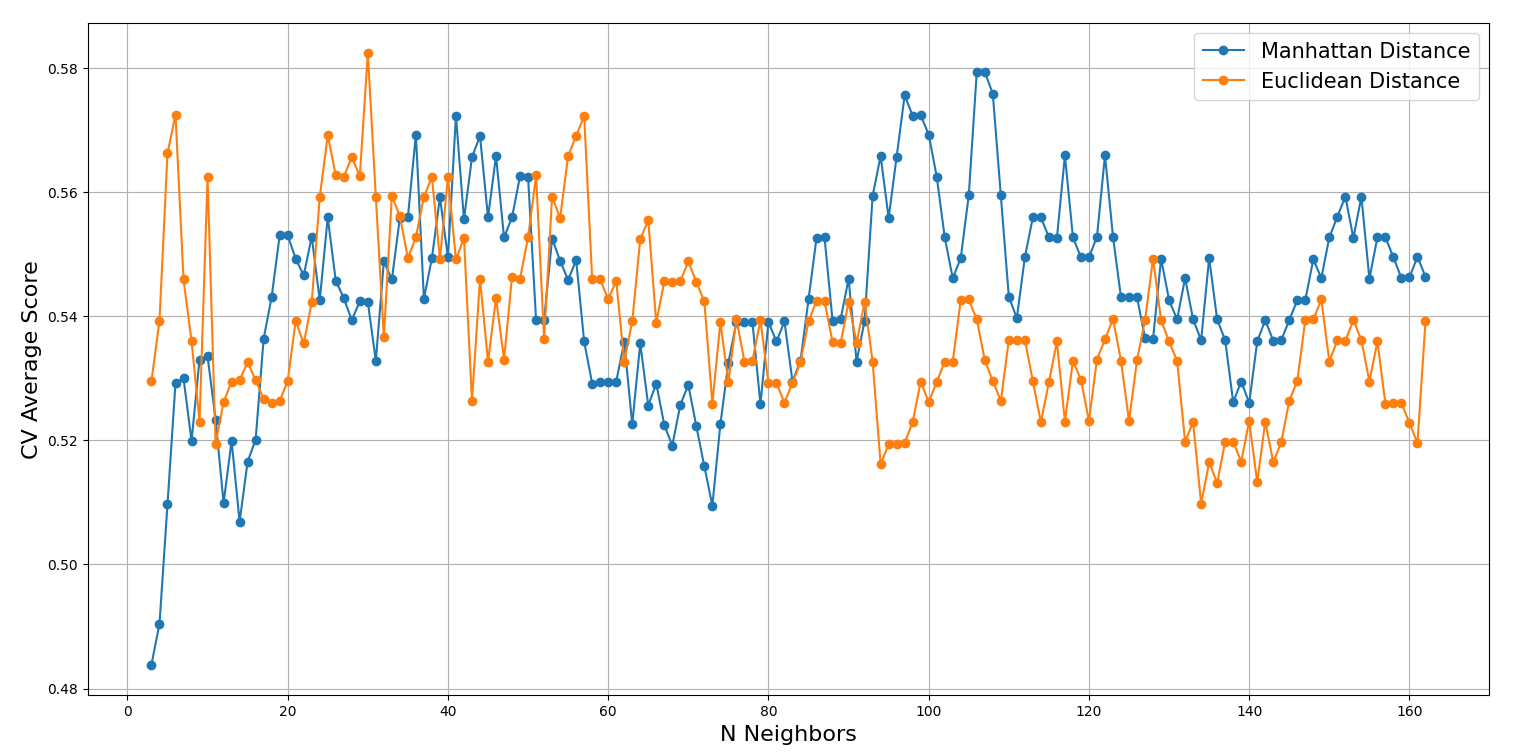
\includegraphics[scale=0.35]{knnCV.png}
		\caption{Grafico dell'andamento della media dell'accuratezza per ogni valore dell'iperparametro N Neighbors e per ogni tipo di metrica di distanza utilizzata durante l'applicazione della Cross Validation con 10 fold per il modello K-Nearest-Neighbors. Ogni punto è un classificatore con un certo numero di vicini. La linea blu indica l'andamento con la distanza di Manhattan mentre la linea arancione l'andamento con la distanza euclidea.
		} 
		\label{fig:knnCV}
	\end{center}
\end{figure}

Quello che si può notare dalla figura è che inizialmente con pochi vicini la distanza euclidea risulta essere migliore nella fase di training nel \emph{validation} \emph{set} ma con l'aumentare del numero dei vicini la distanza di Manhattan ottiene risultati migliori. Secondo la Cross Validation i parametri migliori sono stati 30 come numero di vicini e la distanza euclidea come metrica della distanza da utilizzare. L'accuratezza ottenuta nel \emph{validation} \emph{set} è stata di 0.582.
Nella fase di predizione si sono ottenuti le predizioni mostrate nella Figura \ref{fig:knnpre} con le relative metriche presentate nella Figura \ref{fig:knnmetrics}

\begin{figure}[h]
	\begin{center}
		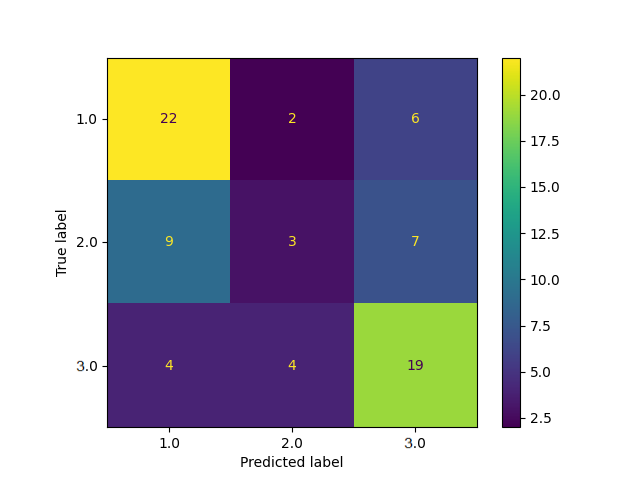
\includegraphics[scale=0.60]{tabknn.png}
		\caption{Tabella di confusione del modello K-Nearest-Neighbors con n\_neighbors = 30 e p = 2. La classe 0.0 indica la vittoria della squadra in casa, la classe 1.0 indica il pareggio tra le due squadre, la classe 2.0 indica la vittoria della squadra ospite.
		} 
		\label{fig:knnpre}
	\end{center}
\end{figure}

Quello che possiamo notare è che i risultati sono discreti. Infatti, l'accuratezza è di 0.58, ciononostante, il modello ha molta difficoltà a riconoscere quando un’osservazione ha come esito il pareggio; infatti, sia la precisione sia la sensibilità sono molto bassi. Ovviamente dato che il modello molto spesso sbaglia a identificare un pareggio la specificità è molto alta. Discreti i risultati ottenuti per gli altri due esiti in termini di precision. Si nota comunque che riesce ad individuare quasi tutte le osservazioni che hanno l'esito vittoria della squadra in casa o vittoria della squadra ospite.
\begin{figure}[h]
	\begin{center}
		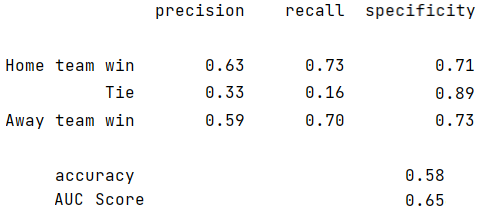
\includegraphics[scale=0.60]{metricknn.png}
		\caption{Grafico delle misurazione durante la fase di predizione del modello K-Nearest-Neighbors con n\_neighbors = 30 e p = 2.
		} 
		\label{fig:knnmetrics}
	\end{center}
\end{figure}

Risulta perciò non particolarmente adatto l'algoritmo K-Nearest-Neighbors per quest'analisi a causa della grande diversità tra partita e partita. Ciononostante, si ottengono discreti risultati tenendo conto del fatto delle poche osservazioni messe disposizione, ovvero 380 partite.
